\documentclass[10pt]{article}
\usepackage{float}
\RequirePackage{eso-pic}
\usepackage{caption}
\captionsetup[table]{labelformat=empty}



\usepackage{geometry}
\geometry{
a4paper,
left=11mm,
right=14mm,
top=37mm,
bottom=14mm,
}



\usepackage{colortbl}
\usepackage{fontspec}
\setmainfont[Ligatures=TeX]{Calibri}



\newcommand\BackgroundPic{%
\put(0,0){%
\parbox[b][\paperheight]{\paperwidth}{%
\vfill
\centering
\includegraphics{MBIE_generic_background.pdf}%
\vfill
}}}



\begin{document}
\thispagestyle{empty}
\AddToShipoutPicture{\BackgroundPic}
\section*{Key Export Statistics\footnotemark - Frozen French Fries\footnotemark }
\today\\
\begin{table}[ht]
\centering
{\scriptsize
\begin{tabular}[t]{p{1.8cm}>{\hfill}p{1.4cm}>{\hfill}p{1.4cm}>{\hfill}p{1.6cm}>{\hfill}p{1.9cm}>{\hfill}p{2cm}>{\hfill}p{1.9cm}>{\hfill}p{1.5cm}}
 \textbf{Country} & \textbf{Yearly Qty} & \textbf{Yearly Value} & \textbf{Yearly Price} & \textbf{3Year CAGR(Qty)} & \textbf{3Year CAGR(Value)} & \textbf{3Year CAGR(Price)} & \textbf{Price Elasticity} \\
\hline
Australia & 42,774 & 51.4 & \$1.2 & 3.2\% & 2.3\% & -0.9\% & -3.7 \\  
Japan & 3,302 & 5.2 & \$1.6 & -3.3\% & 0.5\% & 4\% & -0.8 \\  
Thailand & 1,974 & 3.2 & \$1.6 & -25.5\% & -24.9\% & 0.8\% & -31.1 \\  
French Polynesia & 1,341 & 2.5 & \$1.9 & -9.5\% & -6.6\% & 3.2\% & -3.0 \\  
P.N.G & 834 & 1.3 & \$1.5 & -26.8\% & -26.3\% & 0.7\% & -38.7 \\  
Indonesia & 902 & 1.2 & \$1.3 & 14.7\% & 22.6\% & 6.9\% & 2.1 \\  
Other & 2,745 & 3.9 & \$1.4 & -5.7\% & -5.1\% & 0.7\% & -8.5 \\  
Total & 53,871 & 68.6 & \$1.3 & -0.8\% & -1.6\% & -0.9\% & 0.9 \\  
\hline
\end{tabular}
}
\caption{\scriptsize Top 6 Frozen French Fries Markets for year ending November - 2015: Quantity('000 kg) Value(NZ\$Mill), Price and their last 3-Year Growth Rates}
\end{table}


\vspace{-0.7cm}



   \begin{figure}[H]
   \centering
    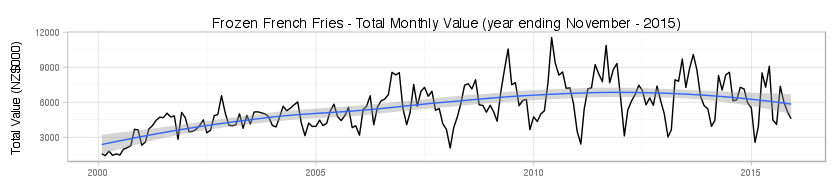
\includegraphics[scale=0.5]{../graphs/monthly_value/frozen_french_fries_monthly_value.png} \
    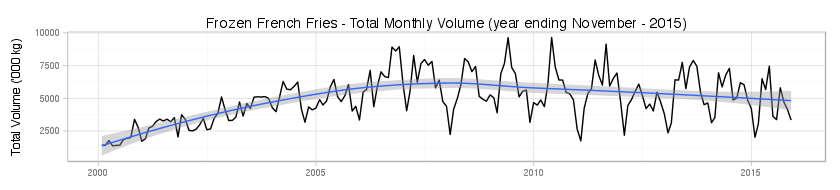
\includegraphics[scale=0.5]{../graphs/monthly_volume/frozen_french_fries_monthly_volume.png} \
    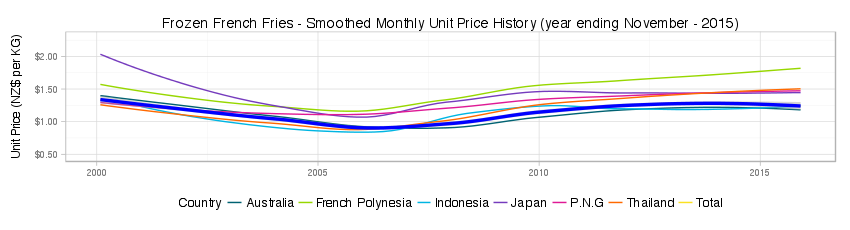
\includegraphics[scale=0.5]{../graphs/smoothed_price/frozen_french_fries_smoothed_price.png} \
    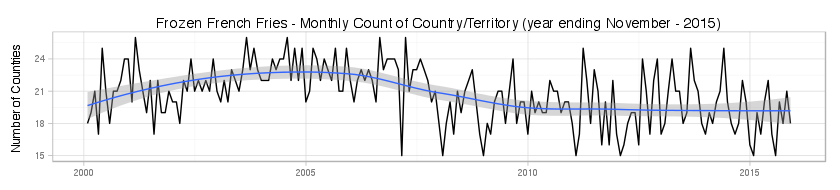
\includegraphics[scale=0.5]{../graphs/monthly_number_countries/frozen_french_fries_monthly_count.png} \
    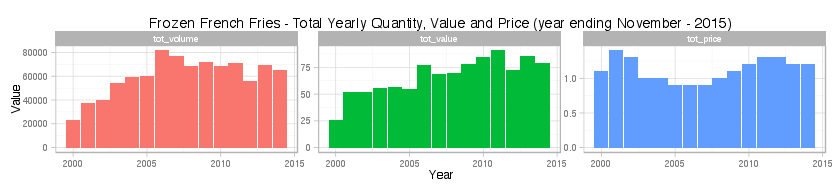
\includegraphics[scale=0.5]{../graphs/yearly_summary/frozen_french_fries_yearly_summary.png} \
   \end{figure}



\footnotetext[1]{Source: Statistics New Zealand - Overseas Merchandise Trade}
\footnotetext[2]{Harmonised System Codes for Frozen French Fries starting with: 200410.}
\end{document}
